\chapter{Notas de codificação aberta (OC)} %Anexo H (novo G) (lista as notas OC e seus respectivos conteúdos)
\label{apendice:h_notas_oc}
\section{Notas de codificação aberta do Grupo 1 (sem PDTI)}
As páginas a seguir contém as 6 notas do tipo OC criadas durante o desenvolvimento da pesquisa sobre o grupo 1.

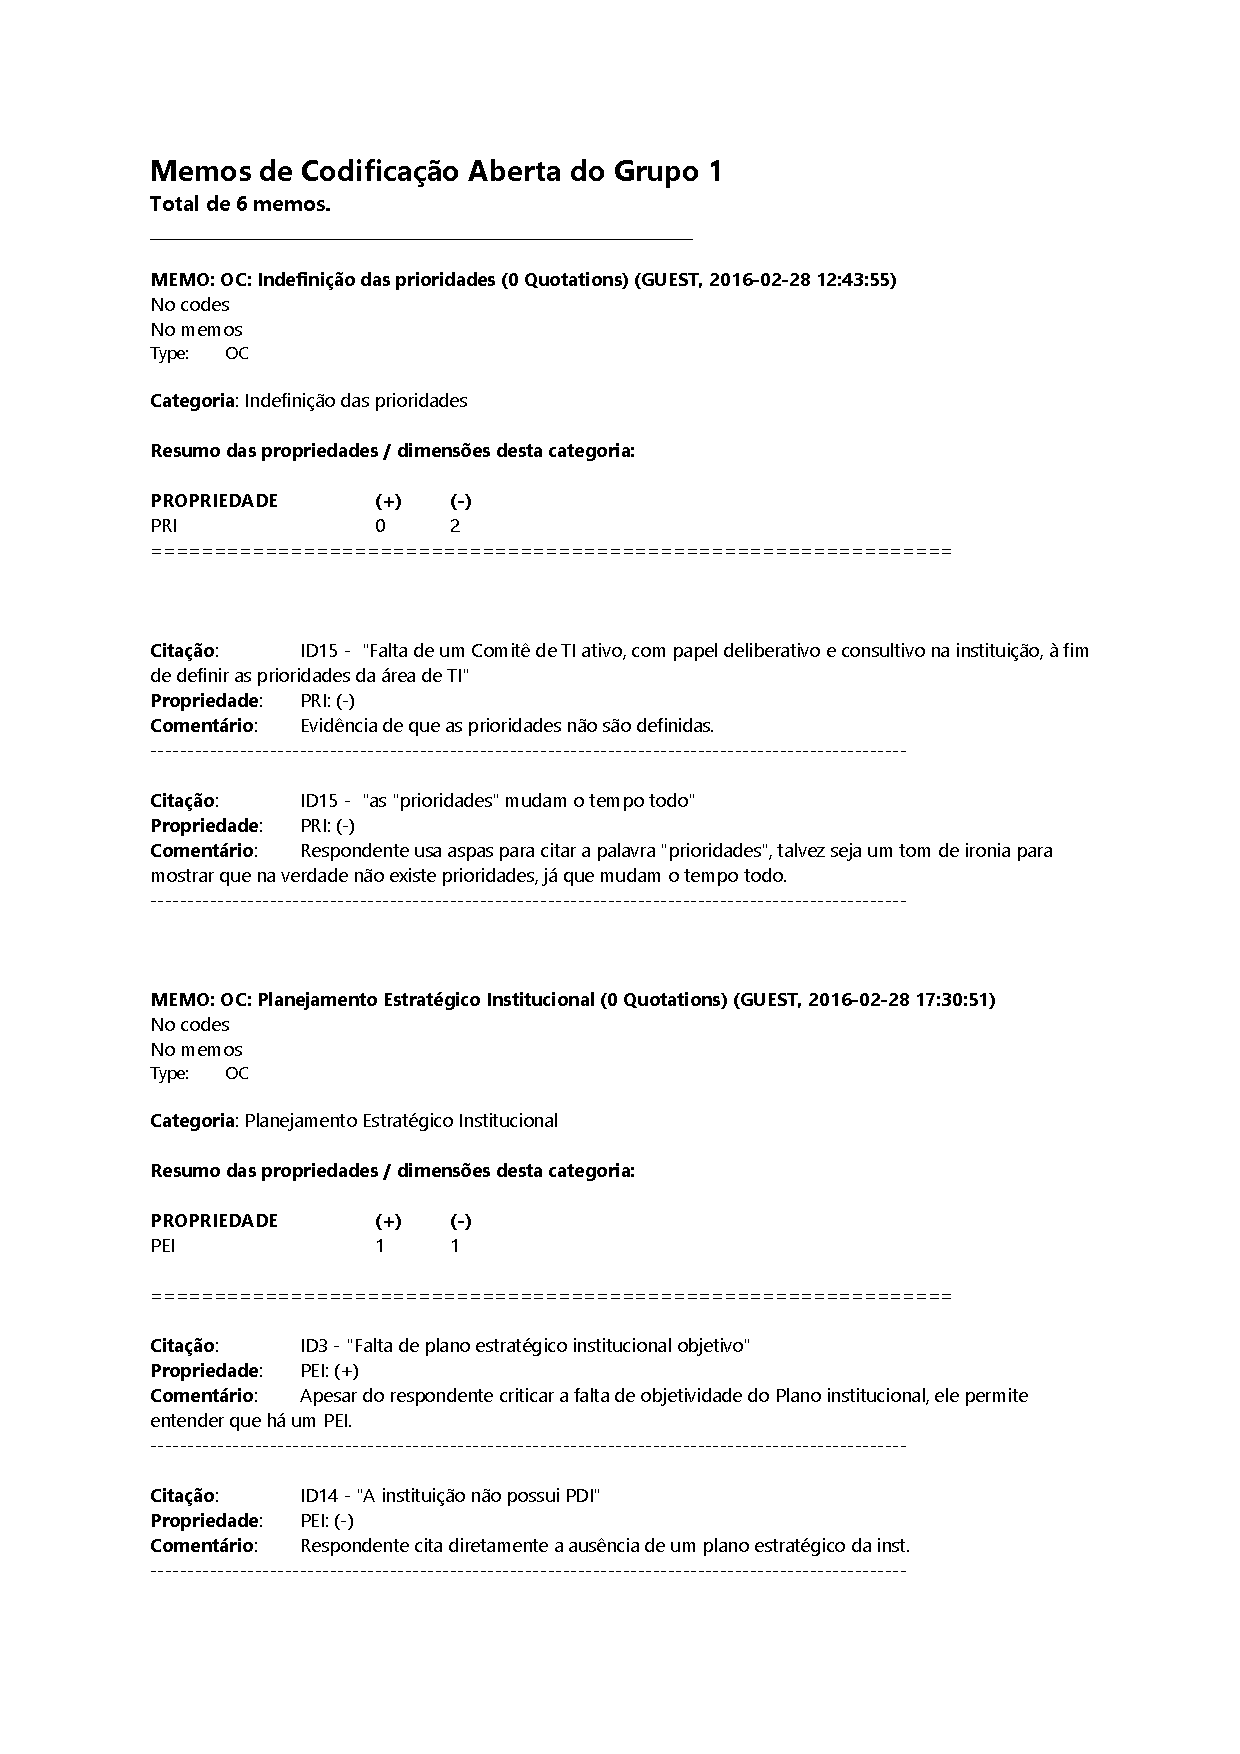
\includepdf[pages=-]{includes/apendiceH_novo_G_OC_g1.pdf}

\section{Notas de codificação aberta do Grupo 2 (com PDTI)}
As páginas a seguir contém as 19 notas do tipo OC criadas durante o desenvolvimento da pesquisa sobre o grupo 2.

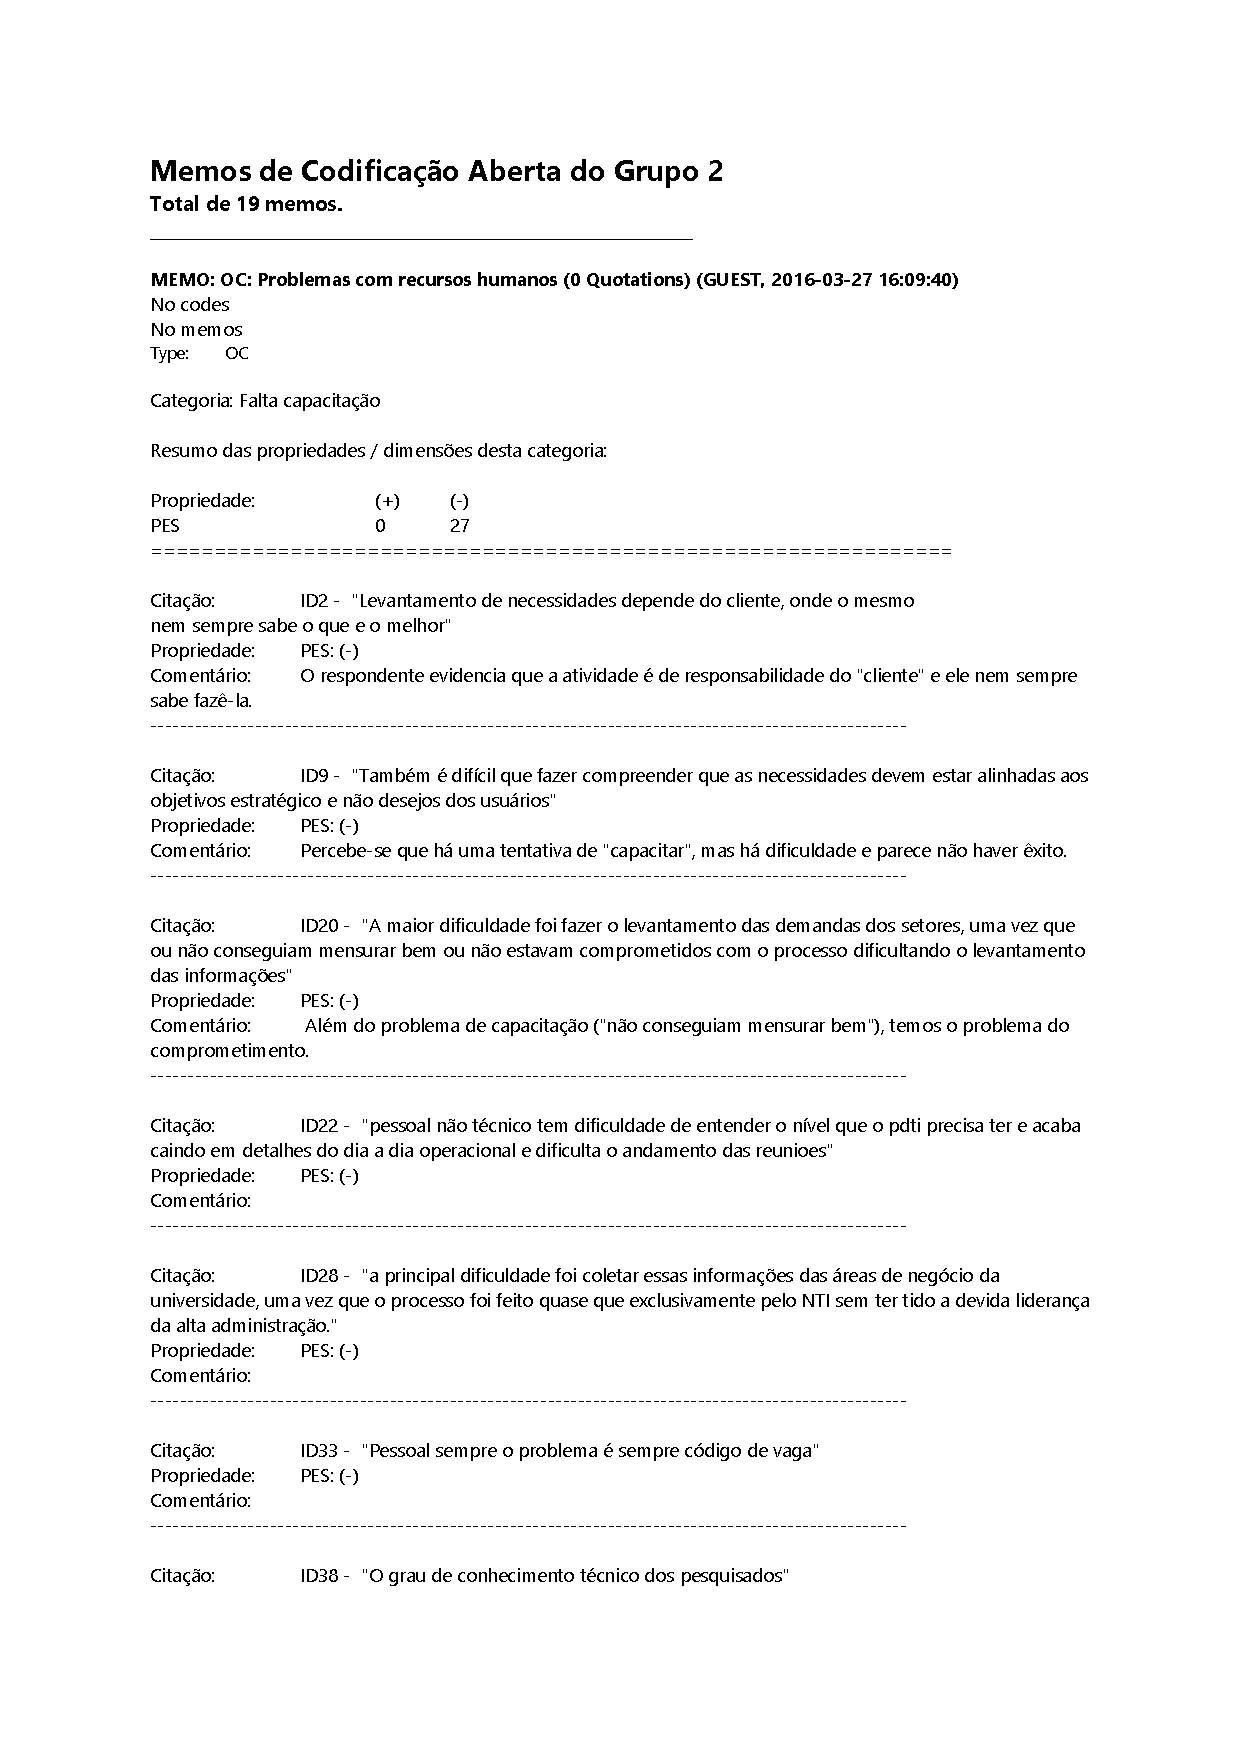
\includepdf[pages=-]{includes/apendiceH_novo_G_OC_g2.pdf}